\section{Desarrollo de software basado en modelos (MBD)} 

\textbf{}\\
El propósito de esta técnica tiene los siguientes 3 objetivos básicos:

\begin{flushleft}

\begin{center}
	
	\end{center}
\begin{itemize}
\textbf{1.	El desarrollo de software basado en modelos (MBD) }
La ingeniería de software establece que el problema de construir software debe ser encarado de la misma forma en que los ingenieros construyen otros sistemas complejos, como puentes, edificios, barcos y aviones. La idea básica consiste en observar el sistema de software a construir como un producto complejo y a su proceso de construcción como un trabajo ingenieril. Es decir, un proceso planificado basado en metodologías formales apoyadas por el uso de herramientas. 
En los finales de los años 70 se observó un cambio importante en la filosofía del desarrollo de software, tendiente a solucionar los problemas descriptos arriba. Tom DeMarco en su libro Structured Analysis and System Specification [DeMarco 79] introdujo el concepto de ingeniería de software basada en modelos. DeMarco destacó que la construcción de un sistema de software debe ser precedida por la construcción de un modelo del sistema, tal como se realiza en otros sistemas ingenieriles. De esta forma, el modelo de un sistema provee un medio de comunicación y negociación entre usuarios, analistas y desarrolladores. Actualmente todos los métodos de desarrollo de software han adoptado esta filosofía. Lo que varía de un método a otro es la clase de modelos que deben construirse, la forma de representarlos, manipularlos, etc. El punto de partida en el proceso de desarrollo de software es la construcción de un modelo, el cual actúa como una especificación precisa de los requerimientos que el sistema debe satisfacer.  Un modelo del sistema consiste en una conceptualización del dominio del problema. El modelo  se focaliza sobre el mundo real: identificando, clasificando y abstrayendo los elementos que constituyen el problema y organizándolos en una estructura formal. 

\begin{center}
    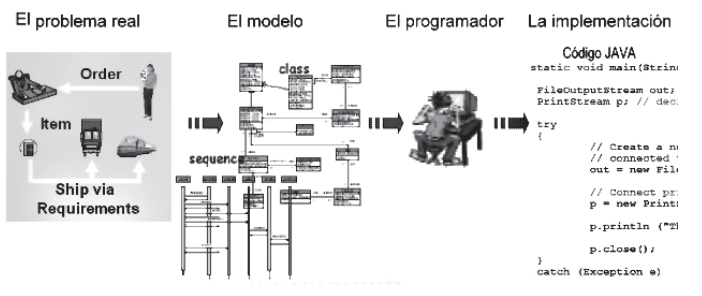
\includegraphics[width=12cm]{./Imagenes/mdd1}
    \end{center}

Actualmente casi todos los métodos de desarrollo de software utilizan modelos. Lo que varía de un método a otro es la clase de modelos que deben construirse, la forma de representarlos y manipularlos. A grandes rasgos podemos distinguir dos tendencias principales: los métodos matemáticos y los métodos diagramáticos.
Métodos Matemáticos:
Estos métodos utilizan lenguajes de especificación de naturaleza matemática, tales como: Z [DB 01], VDM [EF 94], B [BM 00] y OCL [OCL], los cuales permiten demostrar si la especificación cumple ciertas propiedades (ej., consistencia), derivar información implícita a partir de la especificación (ej., usando probadores de teoremas), derivar código automáticamente (ej., aplicando cálculos de refinamientos [BW 98]), verificar formalmente que el software satisface la especificación (ej., aplicando la lógica de Hoare [Hoare 69]).
Métodos Diagramáticos:
Por otra parte, los procesos basados en modelos gráficos –como el UP [JBR 99] con su especialización RUP (Rational Unified process) [Krutchten 00]– constituyen una propuesta más amigable, fácil de utilizar y comprender que los métodos formales. El éxito de estos procesos se basa principalmente en el uso de lenguajes diagramáticos, tales como UML [UML 03] que transmiten un significado intuitivo. A diferencia de las notaciones matemáticas, estos lenguajes diagramáticos son aceptados más fácilmente por los desarrolladores de software.

El ciclo de vida basado en modelos
El proceso de desarrollo de software, como se utiliza hoy en día, es conducido por el diseño de bajo nivel y por el código.
•	La conceptualización y la determinación de los requisitos del usuario 
•	Análisis y descripción funcional 
•	Diseño 
•	Codificación
•	Testeo 
•	Emplazamiento

\begin{center}
    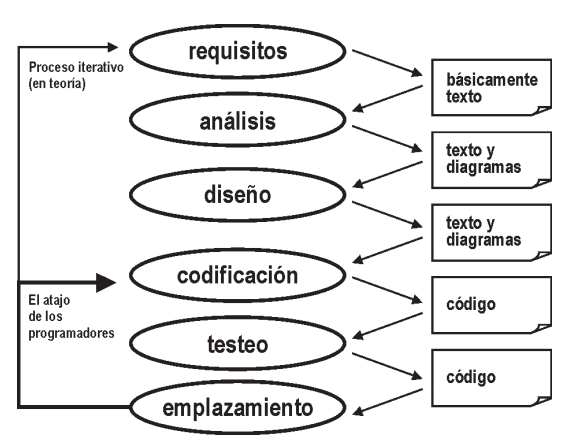
\includegraphics[width=12cm]{./Imagenes/mdd2}
    \end{center}

En las primeras fases se construyen distintos modelos tales como los modelos de los requisitos (generalmente escritos en lenguaje natural), los modelos de análisis y los modelos de diseño (frecuentemente expresados mediante diagramas). Estas fases pueden realizarse de una manera iterativa-incremental o en forma de cascada. En la práctica cotidiana, los modelos quedan rápidamente desactualizados debido al atajo que suelen tomar los desarrolladores en el ciclo de vida de este proceso.
Los problemas del desarrollo basado en modelos 
A continuación, analizamos algunos de los problemas más importantes encontrados durante el desarrollo de software basado en modelos y explicamos sus causas.
El problema de la productividad, el mantenimiento y la documentación: Muchas veces se considera la tarea de la documentación como una sobrecarga adicional. Se cree que escribir código es productivo, pero hacer modelos y documentación no lo es. Dada la complejidad de los sistemas de software actuales, resulta imprescindible contar con documentación en los distintos niveles de abstracción. Planteado así, quedan dos alternativas: o utilizamos nuestro tiempo en las primeras fases del desarrollo del software construyendo la documentación y diagramas de alto nivel y nos preocupamos por mantenerlos actualizados, o utilizamos nuestro tiempo en la fase de mantenimiento descubriendo lo que hace realmente el software.
El problema de la flexibilidad a los cambios tecnológicos: La industria del software tiene una característica especial que la diferencia de las otras industrias. Cada año (o en menos tiempo), aparecen nuevas tecnologías que rápidamente llegan a ser populares (a modo de ejemplo, se pueden listar Java, Linux, XML, HTML, UML, .NET, JSP, ASP, PHP, flash, servicios de Web, etc.). Y muchas compañías necesitan aplicar estas nuevas tecnologías por buenas razones: - Los clientes exigen esta nueva tecnología (por ejemplo, implementaciones para web). - Son la solución para algunos problemas reales (por ejemplo, XML para el problema de intercambio de datos). - La empresa que desarrolla la herramienta deja de dar soporte a las viejas tecnologías y se centra sólo en las nuevas (por ejemplo, el soporte para OMT fue reemplazado por soporte para UML).



\textbf{}\\
\textbf{2.	El desarrollo de software dirigido por modelos (MDD)}

El Desarrollo de Software Dirigido por Modelos MDD (por sus siglas en inglés: Model Driven software Development) se ha convertido en un nuevo paradigma de desarrollo software. MDD promete mejorar el proceso de construcción de software basándose en un proceso guiado por modelos y soportado por potentes herramientas.
Los modelos se van generando desde los más abstractos a los más concretos a través de pasos de transformación y/o refinamientos, hasta llegar al código aplicando una última transformación. La transformación entre modelos constituye el motor de MDD.
Los puntos claves de la iniciativa MDD fueron identificados en [Booch 04b] de la siguiente forma: 
1-	El uso de un mayor nivel de abstracción en la especificación tanto del problema a resolver como de la solución correspondiente, en relación con los métodos tradicionales de desarrollo de software. 
2-	El aumento de confianza en la automatización asistida por computadora para soportar el análisis, el diseño y la ejecución. 
3-	El uso de estándares industriales como medio para facilitar las comunicaciones, la interacción entre diferentes aplicaciones y productos, y la especialización tecnológica.

\begin{center}
    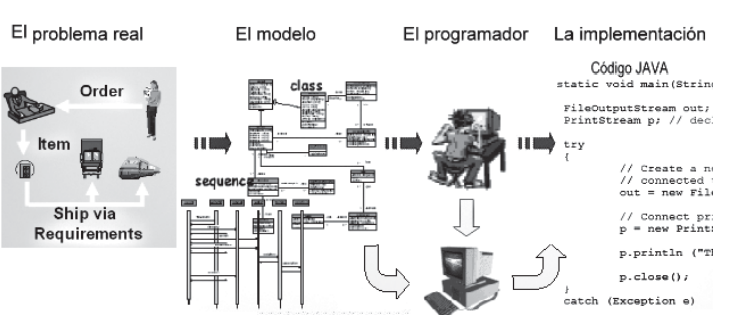
\includegraphics[width=12cm]{./Imagenes/mdd3}
    \end{center}

Abstracción: El enfoque de MDD para incrementar los niveles de abstracción es definir lenguajes de modelado específicos de dominio cuyos conceptos reflejen estrechamente los conceptos del dominio del problema, mientras se ocultan o minimizan los aspectos relacionados con las tecnologías de implementación.
Automatización: La automatización es el método más eficaz para aumentar la productividad y la calidad.
Estándares: MDD debe ser implementado mediante una serie de estándares industriales abiertos.
El ciclo de vida dirigido por modelos
Una de las mayores diferencias está en el tipo de los artefactos que se crean durante el proceso de desarrollo.
MDD identifica distintos tipos de modelos: - modelos con alto nivel de abstracción independientes de cualquier metodología computacional, llamados CIMs (Computational Independent Model), - modelos independientes de cualquier tecnología de implementación llamados PIMs (Platform Independent Model), - modelos que especifican el sistema en términos de construcciones de implementación disponibles en alguna tecnología específica, conocidos como PSMs (Platform Specific Model), - y finalmente modelos que representan el código fuente en sí mismo, identificados como IMs (Implementation Model).

\begin{center}
    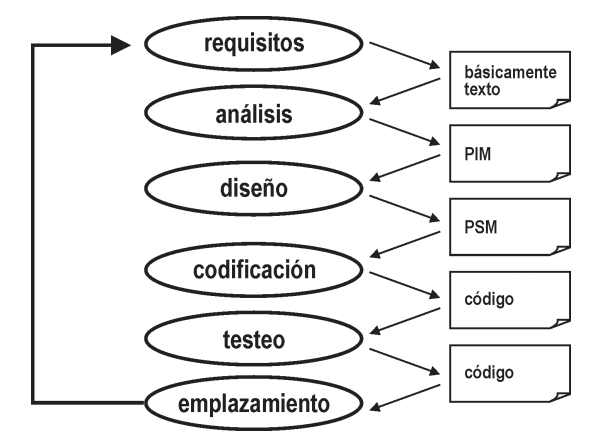
\includegraphics[width=12cm]{./Imagenes/mdd4}
    \end{center}

Muchas herramientas pueden transformar un PSM a código; no hay nada nuevo en eso. Dado que un PSM es un modelo muy cercano al código, esta transformación no es demasiado compleja. Lo novedoso que propone MDD es que las transformaciones entre modelos (por ejemplo de un PIM a PSMs) sean automatizadas.

\begin{center}
    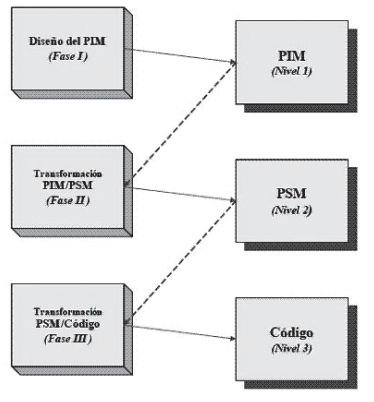
\includegraphics[width=12cm]{./Imagenes/mdd5}
    \end{center}

Orígenes de MDD
MDD es la evolución natural de la ingeniería de software basada en modelos enriquecida mediante el agregado de transformaciones automáticas entre modelos. Por su parte, la técnica de transformaciones sucesivas tampoco es algo novedoso. Podemos remitirnos al proceso de abstracción y refinamiento presentado por Edsger W. Dijkstra en su libro “A Discipline of Programming” [Dijkstra 76] donde se define que refinamiento es el proceso de desarrollar un diseño o implementación más detallado a partir de una especificación abstracta a través de una secuencia de pasos matemáticamente justificados que mantienen la corrección con respecto a la especificación original.
En general estas técnicas de refinamiento se limitan a transformar un modelo formal en otro modelo formal escrito en el mismo lenguaje (es decir, se modifica el nivel de abstracción del modelo, pero no su lenguaje), mientras que MDD es más amplio pues ofrece la posibilidad de transformar modelos escritos en distintos lenguajes (por ejemplo, podemos transformar un modelo escrito en UML en otro modelo escrito en notación Entidad-Relación).
Beneficios de MDD
Incremento en la productividad: MDD reduce los costos de desarrollo de software mediante la generación automática del código y otros artefactos a partir de los modelos, lo cual incrementa la productividad de los desarrolladores.
Adaptación a los cambios tecnológicos: el progreso de la tecnología hace que los componentes de software se vuelvan obsoletos rápidamente. MDD ayuda a solucionar este problema a través de una arquitectura fácil de mantener donde los cambios se implementan rápida y consistentemente, habilitando una migración eficiente de los componentes hacia las nuevas tecnologías.
Adaptación a los cambios en los requisitos: poder adaptarse a los cambios es un requerimiento clave para los negocios, y los sistemas informáticos deben ser capaces de soportarlos.
Consistencia: la aplicación manual de las prácticas de codificación y diseño es una tarea propensa a errores.
Re-uso: en MDD se invierte en el desarrollo de modelos y transformaciones.
Mejoras en la comunicación con los usuarios: los modelos omiten detalles de implementación que no son relevantes para entender el comportamiento lógico del sistema.
Mejoras en la comunicación entre los desarrolladores: los modelos facilitan el entendimiento del sistema por parte de los distintos desarrolladores.
Captura de la experiencia: las organizaciones y los proyectos frecuentemente dependen de expertos clave quienes toman las decisiones respecto al sistema.
Los modelos son productos de larga duración: en MDD los modelos son productos importantes que capturan lo que el sistema informático de la organización hace.
Posibilidad de demorar las decisiones tecnológicas: cuando aplicamos MDD, las primeras etapas del desarrollo se focalizan en las actividades de modelado.


\textbf{}\\
\textbf{3.	Propuestas Concretas para MDD}
Esto es realmente más técnica, porque con buenos hábitos de programación siempre se logra que el proyecto sea modular y reutilizable. Prepararlo para el cambio es una característica que no se consigue siempre y que con TDD si, ya que muchas veces cuando se tiene que cambiar la funcionalidad de la aplicación se tiene que refactorizar código ajeno, trabajar con código complicado, entre otras cosas; en cambio con TDD se tiene la confianza de que cuando se haga cambios no se van a estropear las funcionalidades que ya se tienen. Esto se consigue ya que la forma funcional de TDD es que primero se construye la prueba y luego el código hace que todo lo que surja en él ya este testeado, así que cualquier cambio que se vaya a introducir estará cubierto por los tests y si llegas a dañar algo alguno de ellos reaccionara cuando se ejecuten.
\textbf{}\\
Todo esto cambia un poco la mentalidad tradicional que es: primero analizar los requisitos, luego hacer un diseño completo y profesional, después empezar a codificar y por último testear. Lo que hay que hacer es que, en vez de planear tareas pensar en ejemplos y datos concretos, ya que en eso se basa los test, tener parámetros de entrada y de salida y luego ver si la respuesta es lo que se esperaba.
Si con TDD consigues tener en las especificaciones o requisitos una lista de ejemplos muy completa, que sean concretos, que elimine cualquier tipo de ambigüedad y que se puedan transformar en pruebas, al final tendrás una batería de tests que te cubrirán todas las funcionalidades y el código resultante estará 100\% cubierto por dichos test.




\end{itemize} 